\documentclass[final,t]{beamer}

% poster template
\usepackage[orientation=portrait,size=a0,scale=1.4,debug]{beamerposter}
\usetheme{es}
\usepackage[utf8]{inputenc}
\usepackage{fontspec}
\usepackage{fontawesome}
% use ttf font, see  http://tex.stackexchange.com/questions/239801/fontawesome-scaling-deedy-resume-pgfplots-axis-xetex-luatex-issues
% \newfontfamily{\FA}[Path = fonts/]{fontawesome-webfont}
\newfontfamily{\FA}[Path = fonts/]{FontAwesome-1000upm}
\usepackage{color}
\usepackage{natbib}

% add circle to enumitem
\usepackage{enumitem}
\setitemize{label=\usebeamerfont*{itemize item}%
\usebeamercolor[fg]{itemize item}
\usebeamertemplate{itemize item}
}
\setbeamertemplate{itemize item}{\small\raise1.25pt\hbox{$\blacktriangleright$}}

\usepackage{tikz}
\newcommand*{\numberingI}[1]{%
\footnotesize\protect\tikz[baseline=-3px]%
\protect\node[fill=none,shape=circle,draw,inner sep=1.5pt,line width=1mm, color=blue, font=\bf, yshift=0.45cm](n1){\large #1};
}

% caption size
\usepackage[margin=1cm]{caption}
\captionsetup{font=normalsize, labelfont={color=blue,bf, normalsize}}



% document meta
\title{Ecotoxicology is not normal.}
\author{Eduard Sz\"ocs, Ralf B. Sch\"afer}
\institute{Institute for Environmental Sciences, University of Koblenz-Landau}
\footer{\faDownload~Paper, poster \& source code here: \color{alu1}{https://github.com/EDiLD/usetheglm}}


%------------------------------------------------------------------------------
\begin{document}
\begin{frame}{}
\begin{columns}[t]
%-----------------------------------------------------------------------------
%                                                                     COLUMN 1
% ----------------------------------------------------------------------------
\begin{column}{.48\linewidth}

    % Problem
    \begin{exampleblock}{Most eco(toxico)logical data is not normally distributed}
        \begin{center}
          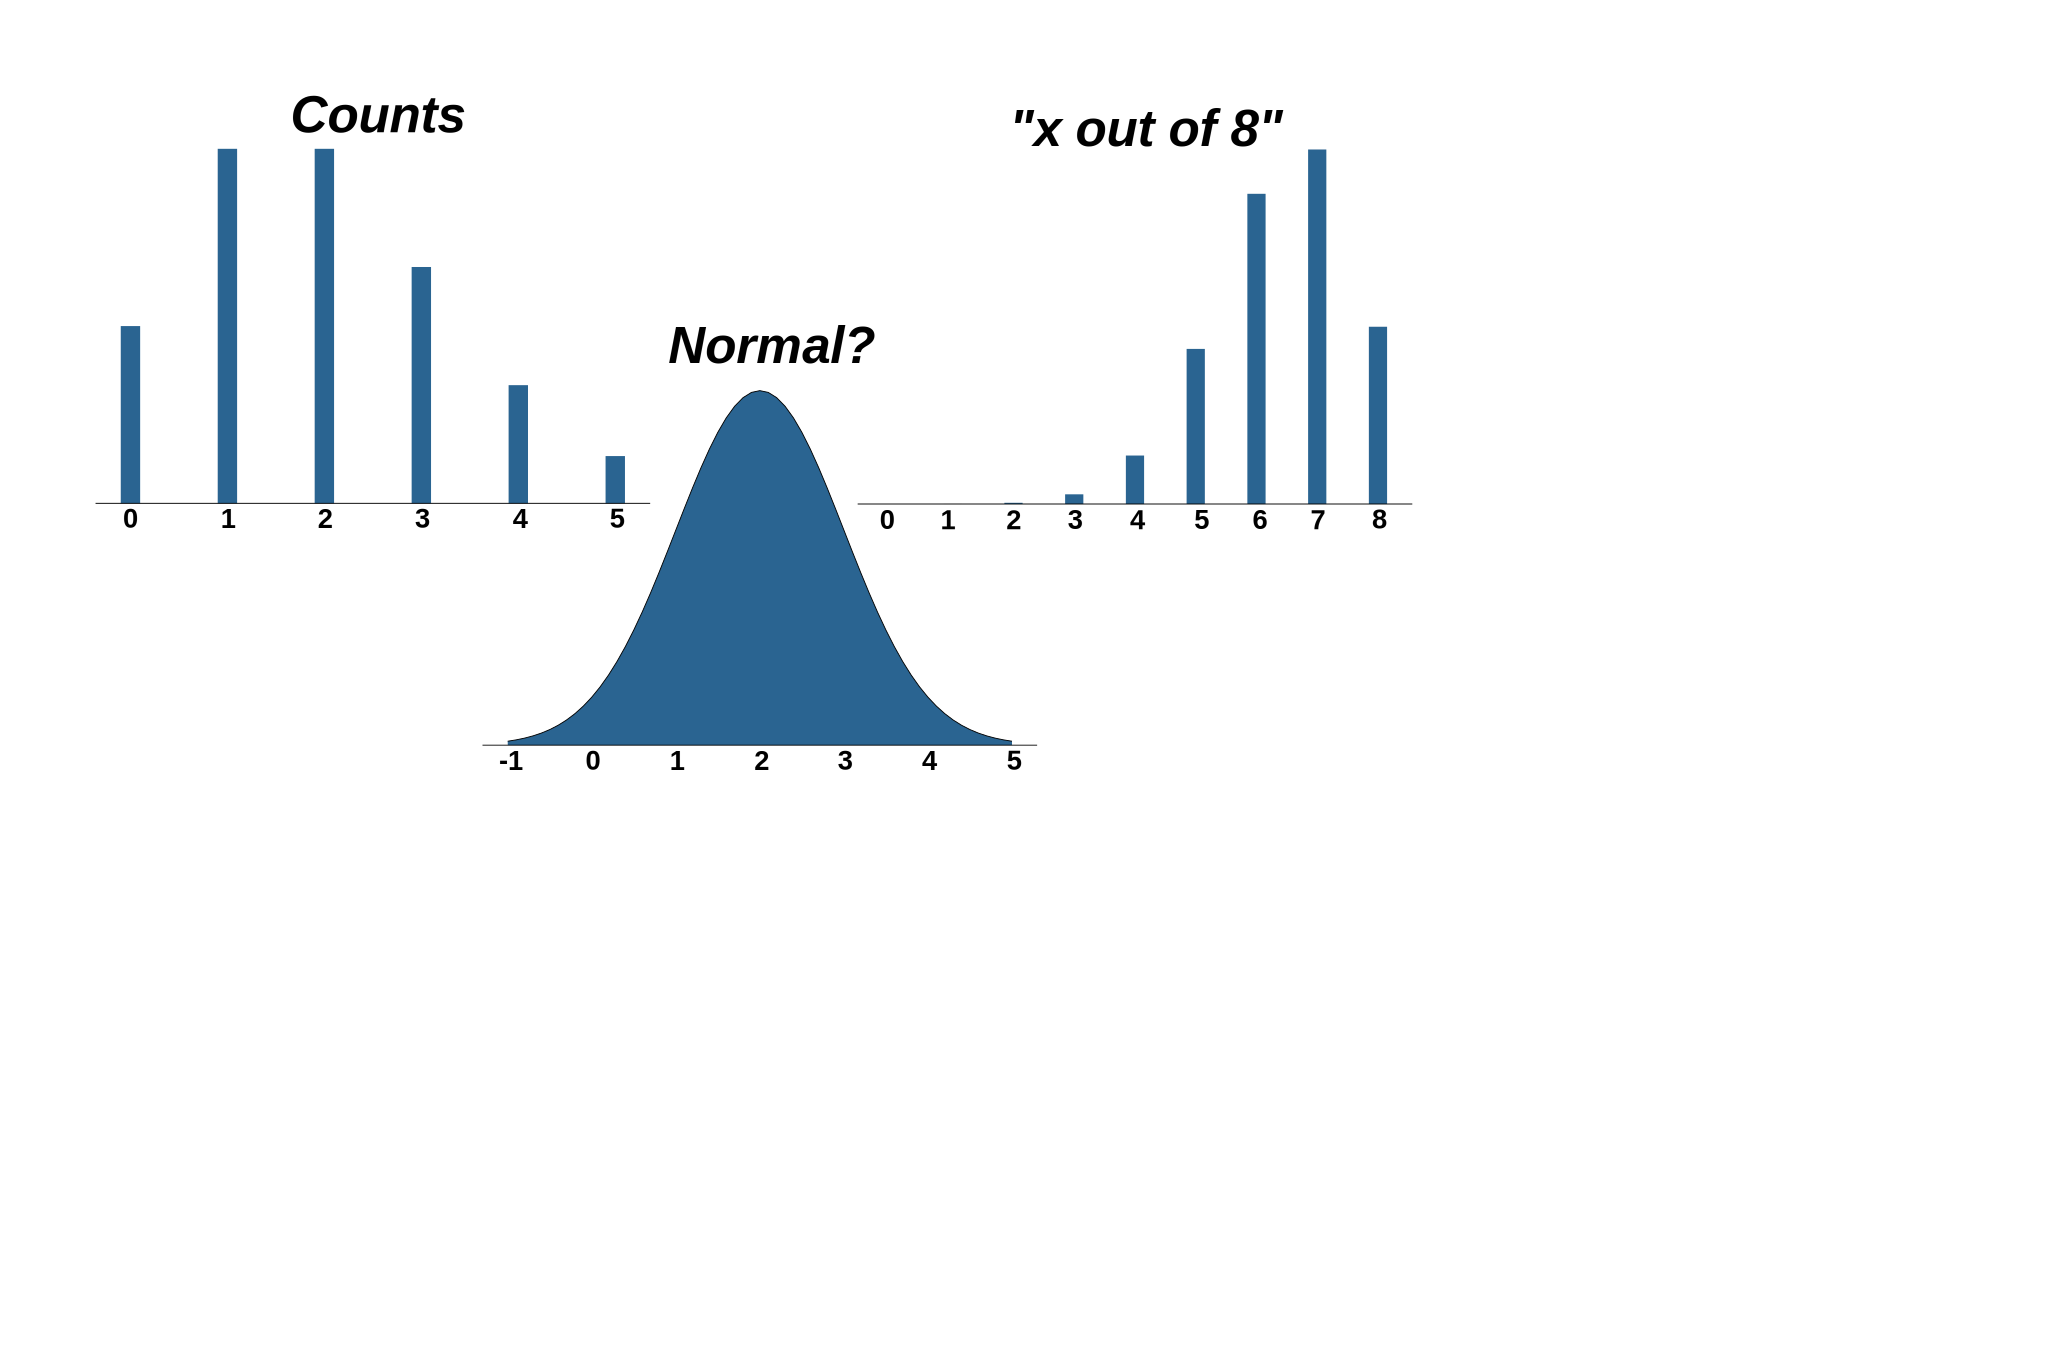
\includegraphics[width=0.8\linewidth]{fig/distr.png}
        \end{center}

        \begin{itemize}
            \item Usually analysed by using \\[0.5ex]
                \begin{itemize}[label=$-$]
                    \item transformations (e.g. $log(Ax + C)$, $x^{0.5}, arcsine~x^{0.25}$) for linear model \cite{newman_quantitative_2012}
                    \item non-parametric methods \cite{wang_making_2011}
                \end{itemize}
                \vskip1ex
            \item \emph{Generalized Linear Models} (GLM) can directly model such data
            \item Can GLMs enhance inference in ecotoxicology?
        \end{itemize}
    \end{exampleblock}


    \begin{block}{Methods: Simulation study}
    \setbeamercolor{itemize item}{fg=blue}
    \begin{columns}[T]
    \begin{column}{.48\linewidth}
        \begin{itemize}
            \item Simulated overdispersed counts
            \item One-factorial design, 50\% effect
            \item Variates:
                \begin{itemize}[label=$-$]
                    \item Number of replicates
                    \item Abundance
                \end{itemize}
                \vskip1ex
            \item Methods:
                \begin{itemize}[label=$-$]
                    \item linear model on transformed data
                    \item GLM (Poisson, negative binomial, quasi-Poisson)
                    \item Kruskal-Wallis / pairwise Wilcoxon
                \end{itemize}
                \vskip1ex
            \item Endpoints:
                \begin{itemize}[label=$-$]
                    \item Global Treatment effect (F-Test, LR-Test)
                    \item LOEC (Dunnett contrasts)
                \end{itemize}
            \end{itemize}
        \end{column}
        \begin{column}{.48\linewidth}
            \begin{figure}
             \includegraphics[width=\linewidth]{fig/sim.png}
             \caption{A realised simulation. N = 3, mean  = 32, effect = 50\%}
             \end{figure}
        \end{column}
        \end{columns}
    \end{block}

    \begin{block}{Results: Claiming an effect when there is none (Type I error)}
        \begin{figure}
             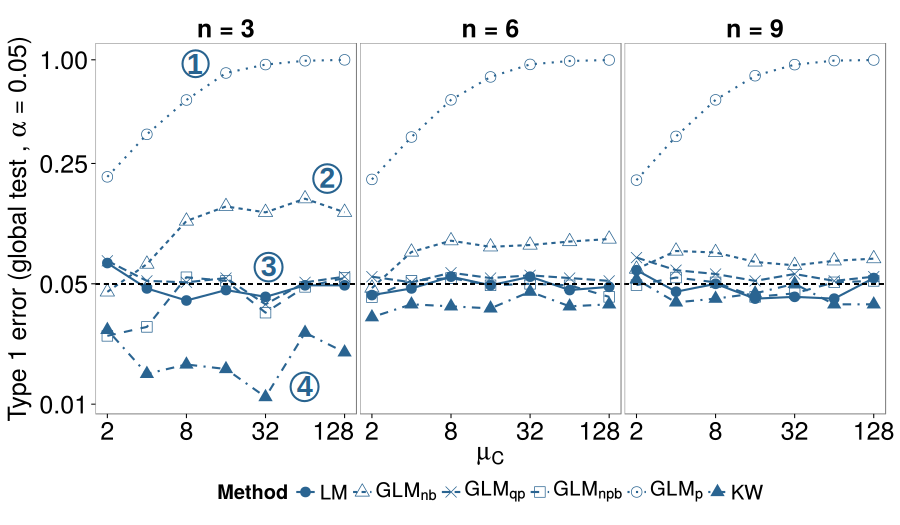
\includegraphics[width=.95\linewidth]{fig/T1.png}
             \caption{Type I errors for testing a global treatment effect. }
         \end{figure}
         \vskip2ex
         %enumitem does not play well with beamer, fix symptoms: Horizontal scale (minpage) and alignments (centered, makebox)
        \noindent\makebox[\textwidth][c]{%
         \begin{minipage}{0.95\linewidth}
         \begin{enumerate}[label=\numberingI{\arabic*}, itemindent=0cm, itemsep = 1.5ex]
            \item Poisson GLM does not fit to the data (overdispersion) and overestimates significance
            \item Increased Type I errors for negative binomial GLM
            \item Negative binomial GLM + bootstrap gives correct levels. Quasi-Poisson GLM and Linear model give appropriate error levels.
            \item Kruskal-Wallis test  shows low Type I error (loses power)
         \end{enumerate}
        \end{minipage}
         }
    \end{block}

\end{column}


%-----------------------------------------------------------------------------
%                                                                     COLUMN 2
% ----------------------------------------------------------------------------
\begin{column}{.48\linewidth}

    \begin{block}{Results: How often is a reduction of 50\% detected? (Power)}
        \begin{figure}      
             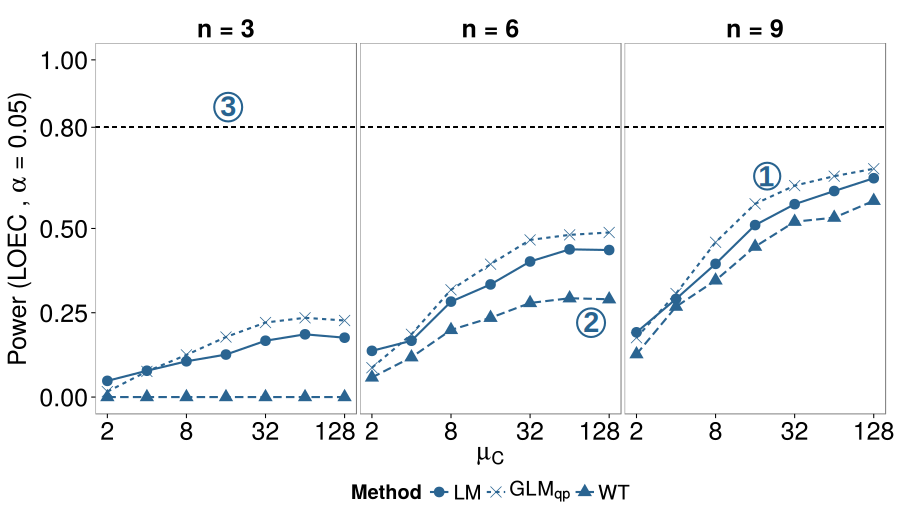
\includegraphics[width=.95\linewidth]{fig/Power.png}
             \caption{Power to detect LOEC. Only methods wtih appropriate Type I errors are displayed.}
         \end{figure}

         \vskip2ex
         \noindent\makebox[\textwidth][c]{%
         \begin{minipage}{0.95\linewidth}
          \begin{enumerate}[label=\numberingI{\arabic*}, itemindent=0cm, itemsep = 1.5ex]
            \item Quasi-Poisson GLM has greater power then the linear model on transformed data
            \item Pairwise Wilcoxon has reduced power
            \item  Low power to detect LOEC at a reduction of 50\%  for common mesocosm designs
         \end{enumerate}
         \end{minipage}
         }
    \end{block}


    \begin{block}{Power estimation app}
    \setbeamercolor{itemize item}{fg=blue}
    \begin{itemize}
        \item \emph{For "a priori"} power calculations
        \item web based, easy to use, for one factorial designs
        \item Currently hostet at \faGlobe~\textbf{\textcolor{blue}{http://52.28.43.83/shinypower/}}
        \vskip2ex
    \end{itemize}
        \begin{center}
          \includegraphics[width=0.7\linewidth]{fig/shinytox.png}
        \end{center}
        \vskip -0.5cm
    \end{block}
  
    % Conclusions
    \begin{alertblock}{Conclusions}
        \begin{itemize}
            \item Low power at common experimental designs (NOEC !?)
            \item Change your model, not your data!
            \item GLM increases Power for  count and binomial data
            \item Negative binomial GLM not recommended (but see bootstrap).
            \item GLMs for multivariate data?  See \cite{szocs_analysing_2015} for a comparison with PRC.
        \end{itemize}
    \end{alertblock}

        % References
    \begin{block}{References}
    \vskip -0.5cm
        \small     
        \bibliographystyle{plain}
       \bibliography{references}   
       \vskip -0.5cm
    \end{block}

    \begin{block}{Contact}
    \vskip -0.5cm
    \normalsize
    \faEnvelope ~\textbf{szoecs@uni-landau.de} \hfill  \faTwitter ~@EduardSzoecs \\[1ex]
    \faGlobe ~\textbf{http://edild.github.io/}   \hfill \faTwitter ~@LandscapEcology \\[1ex]
    \hfill \faGithub ~ @EDiLD 
    \vskip -0.5cm
    \end{block}

\end{column}
\end{columns}

\end{frame}
\end{document}
